\subsection{Erste Datensammlung und manuelle Aufbereitung}
Für eine möglichst gute Datengrundlage wurde an einer geraden Straße Aufnahmen von insgesamt 21 vorbeifahrenden Kfz gemacht, sowohl von dicht aufeinanderfolgenden, als auch einzelnen Fahrzeugen. Als Aufnahmegerät wurde ein Smartphone mit integrierter Rekorder-App verwendet. Die zusammenhängende Aufnahme aller Fahrzeuge wurde anschließend von Hand in einzelne Abschnitte unterteilt und als WAV-Audiodateien gespeichert. \draftred{Dieses unkomprimierte Format wurde gewählt, um die Implementierung der Datenanalyse zu erleichtern.}\todo[inline]{Andere Begründung?} %todo

\subsection{Analyse der Audiodaten via Dopplereffekt}
Da im Phy\-sik-Unter\-richt eine Abituraufgabe zur Geschwindigkeitsbestimmung eines Rennwagens mittels Differenz der Frequenz bei Annäherung und Entfernung behandelt wurde, ist das der erste verfolgte Ansatz. Es erscheint zudem einfach, die Geschwindigkeit akkurat zu ermitteln, da selbst ein Mensch eindeutige Frequenzveränderungen hören kann, beispielsweise bei einem vorbeifahrenden Krankenwagen mit Martinshorn. Allerdings muss bei normalen Kfz das Reifengeräusch anstelle des Martinshorns verwendet werden, da dieses mit Abstand die lauteste Geräuschquelle des Straßenverkehrs ist.

Wenn der Abstand des vorbeifahrenden Fahrzeugs zum Beobachter vernachlässigt und von konstanter Bewegungsgeschwindigkeit ausgegangen wird, können folgende Formeln zur Berechnung der Geschwindigkeit verwendet werden:

\[
    f_{1} = f_{0} * \frac{c}{c - v}
    \quad\text{und}\quad
    f_{2} = f_{0} * \frac{c}{c + v}
\]

Dabei ist \(f_{1}\) die vom Beobachter registrierte Frequenz bei Annäherung und \(f_{2}\) die Frequenz bei Entfernung des Fahrzeugs. Die Konstante \(c\) wird mit \(c = 343\frac{m}{s}\) als Schallgeschwindigkeit in Luft angenommen. Durch Messung beider Frequenzen kann das Frequenzverhältnis \(k = \frac{f_{1}}{f_{2}}\) berechnet und nach \(v\) umgestellt werden:

\begin{equation*}
    \begin{split}
        k & = \frac{f_{0} * \frac{c}{c - v}}{f_{0} * \frac{c}{c + v}} \\
        k & = \frac{c + v}{c - v} \\
        & \Leftrightarrow \\
        v & = \frac{k - 1}{k + 1} * c
    \end{split}
\end{equation*}

\begin{figure}[h]
    \centering
    \import{rsc/plots/f-t-plot/}{frequenz-zeit-plot.tex}
    \caption{Beispielhafter Frequenzverlauf bei vorbeifahrendem Fahrzeug}
    \label{fig:frequencyplot}
\end{figure}

Des Weiteren ist mit dem Dopplereffekt die Entfernungsbestimmung von Mikrofon und Fahrzeug möglich, indem die Änderungsgeschwindigkeit der Frequenz analysiert wird. Hierbei gilt: je größer die Änderungsrate, desto dichter sind Fahrzeug und Beobachter (siehe \autoref{fig:frequencyplot}).

\subsubsection{Verwendung der Reifengeräusche}

Für einen ersten Überblick wurden die Audio-Abschnitte in einen Spektrumanalysator geladen. Die Ergebnisse der visuellen Analyse sind in \autoref{img:spectrumanalyzer} dargestellt.

\begin{figure}[h]
    \begin{subfigure}{.5\textwidth}
        \centering
        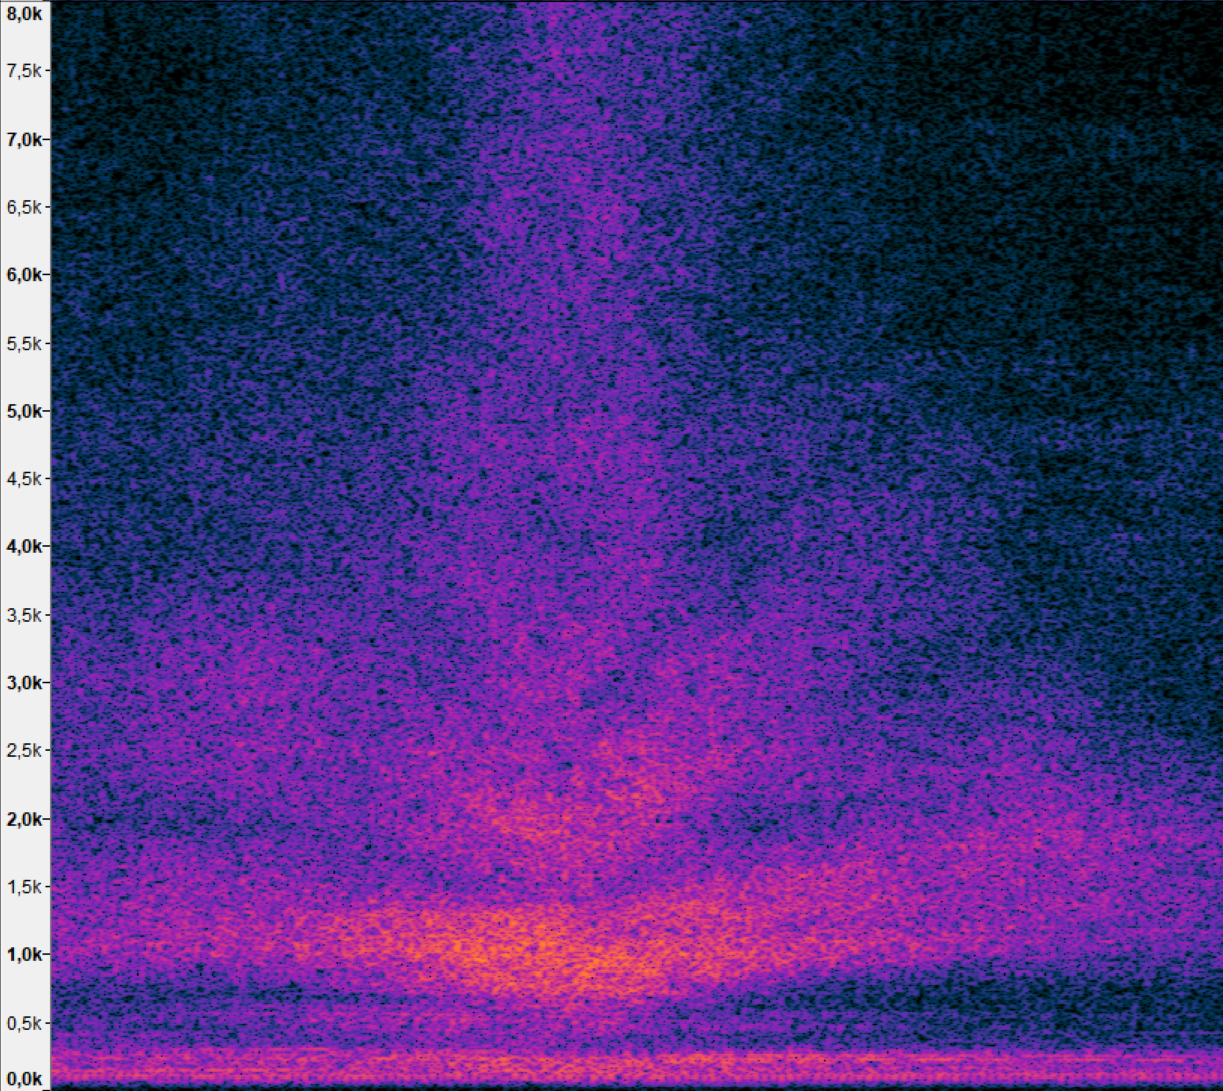
\includegraphics[width=.8\linewidth]{Frequenzen}
        \caption{Spektrogramm}
    \end{subfigure}
    \begin{subfigure}{.5\textwidth}
        \centering
        \includegraphics[width=.8\linewidth]{Tonhöhe(EAC)}
        \caption{Tonhöhe (EAC)}
        \label{img:spectrum_b}
    \end{subfigure}
    \caption{Ergebnisse Spektrumanalysator Reifengeräusche}
    \label{img:spectrumanalyzer}
\end{figure}

\autoref{img:spectrum_b} wurde nachbearbeitet. Die pinkfarbene Linie zeigt den Verlauf der Tonhöhe über Zeit und kann als Frequenzgraph interpretiert werden. Ab der tiefsten Stelle des Graphen ist das vorbeifahrende Kfz am nächsten zum Mikrofon.

Beim Vergleich mit einem theoretisch berechneten Frequenzgraph (\autoref{fig:frequencyplot}) fällt auf, dass die aufgenommene Frequenz der Reifengeräusche vor Vorbeifahren (in der Beispielabbildung bei \(t = 10 s\)) nicht höher ist als nach dem Vorbeifahren, sondern bei niedrigerem Abstand geringer ist. Es konnte keine wissenschaftliche Erarbeitung dieses Phänomens gefunden werden, am wahrscheinlichsten ist jedoch eine Reflexion der akustischen Wellen am Boden, die mit den direkt zum Mikrofon laufenden Wellen interferieren und somit hohe Frequenzen auslöschen. Aufgrund dieser unklaren Messergebnisse kann dieser Ansatz jedoch nicht weiterverfolgt werden.

\subsubsection{Verwendung der Motorgeräusche}

\begin{figure}[h]
    \centering
    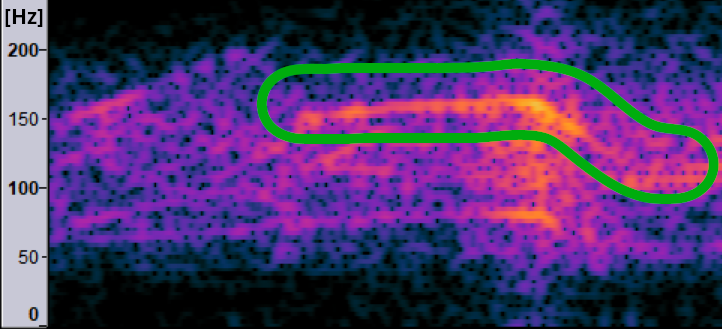
\includegraphics[width=.6\linewidth]{SpektrogrammMotor}
    \caption{Spektrogramm Motorgeräusche}
    \label{fig:spectrum_motor}
\end{figure}

Nachdem sich die Reifengeräusche als unbrauchbar erwiesen haben, ist nun der nächste Ansatz, die Motorgeräusche aufgrund der eindeutigeren Tonhöhe -- anstatt eines Rauschens -- zu analysieren. Hierfür wird ein Tiefpass mit einer Grenze von \(150 Hz\) auf die Audiospur gelegt, um jegliche Reifengeräusche herauszufiltern. Bei der manuellen Analyse stellt sich jedoch heraus, dass selbst die besten Aufnahmen unbrauchbar sind: Der in \autoref{fig:spectrum_motor} grün umrandete Frequenzverlauf stellt die aufgenommenen Motorgeräusche dar, bei denen die Dopplerverschiebung sichtbar ist. Zwar beinhaltet die Aufnahme vor dem Vorbeifahren des Kfz eindeutige Motorgeräusche, allerdings gibt es keine Messpunkte bei Entfernung des Fahrzeugs (hinter dem „Knick“ im Spektrogramm verschwindet die helle, gelbe Linie). Die Motorgeräusche, die direkt mit der Motordrehzahl zusammenhängen, konnten vom verwendeten Handymikrofon gar nicht aufgezeichnet werden, vermutlich unterläge es jedoch den gleichen Einschränkungen wie die aufgezeichneten Oberwellen. Somit kann auch diese Variante der Geschwindigkeitsbestimmung nicht verwendet werden.

\subsection{Analyse der Audiodaten via Lautstärkeänderung}


Das morgen im Freien irgendwie ausprobieren
-> Schallquelle nicht gerichtet (z.B. Lautsprecher zeigt nach oben, also in die Vertikale)
-> Die Abstandsmessung erfolgt in der Horizontalen